%===============================================================================%
\chapter{Applications and Visualisations} \label{chapter:application}
%===============================================================================%

%300 words on how the data can be used.
\lipsum[1-2]

%-------------------------------------------------------------------------------%
\section{Footfall Landscape of United Kingdom}
%-------------------------------------------------------------------------------%
% how the data can be used in understanding the nature of the places they are installed. Aggregated to different level.
\lipsum[3]
\subsection{UK footfall index}
% Combining them together to have and index UK. How footfall has gone up or down every week compared to last week or compared to last year.
\lipsum[1]

\begin{figure*}
  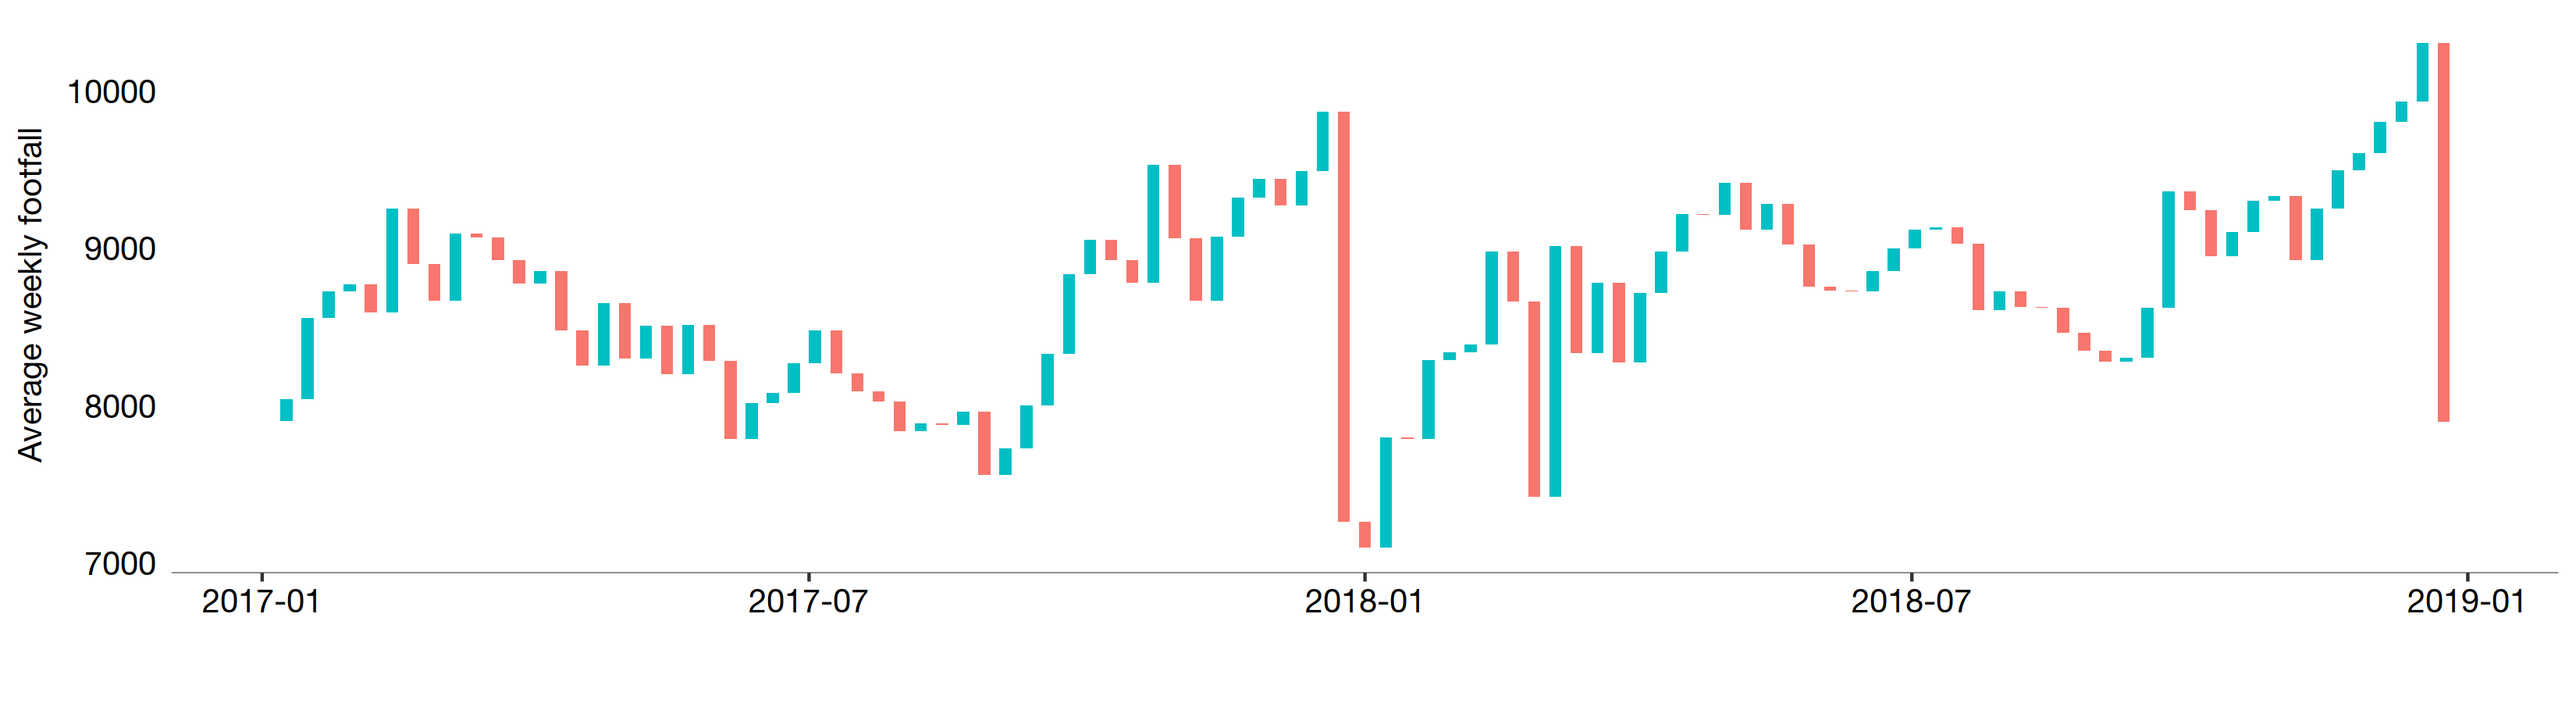
\includegraphics[trim={0 25 0 10},clip]{images/applications-footfall-index.png}
  \caption{}
  \label{}
\end{figure*}

\subsection{City wise indices}
% The footfall profiles in a day can be used to see how different cities work differently.
\lipsum[1-2]

\begin{figure*}
  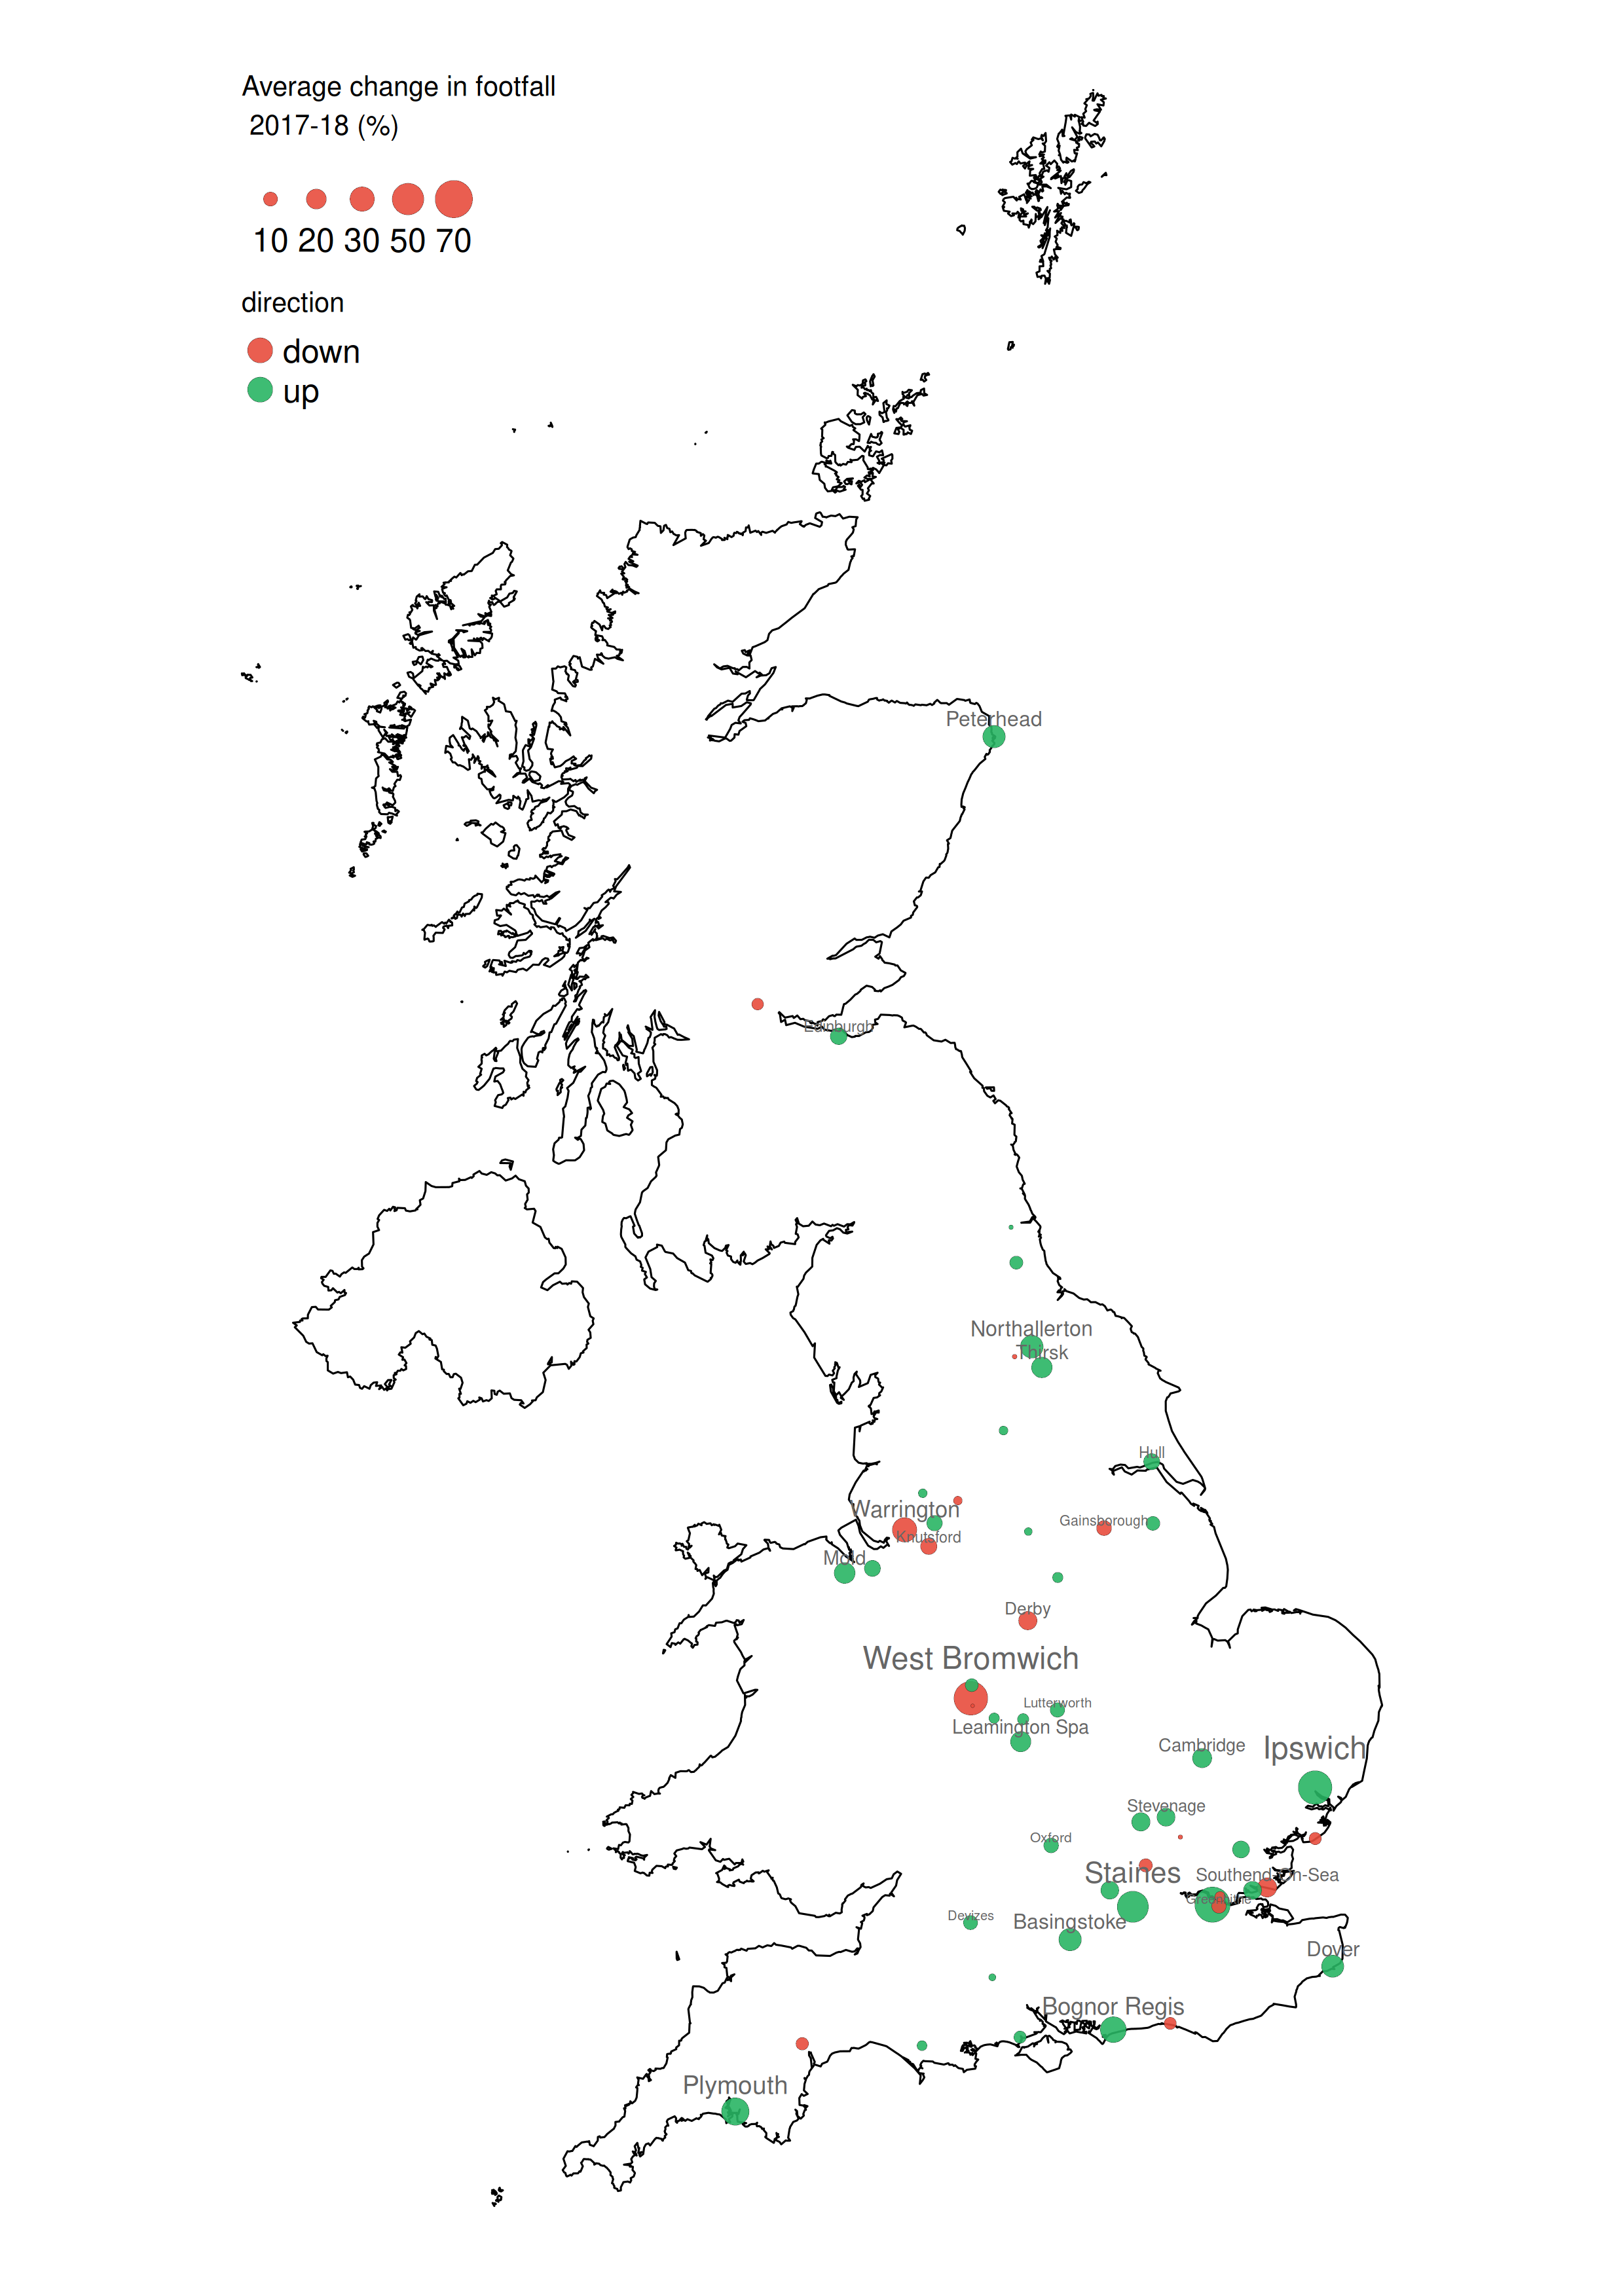
\includegraphics[trim={0 0 0 0},clip]{images/applications-cities-rank.png}
  \caption{}
  \label{}
\end{figure*}

\begin{figure*}
  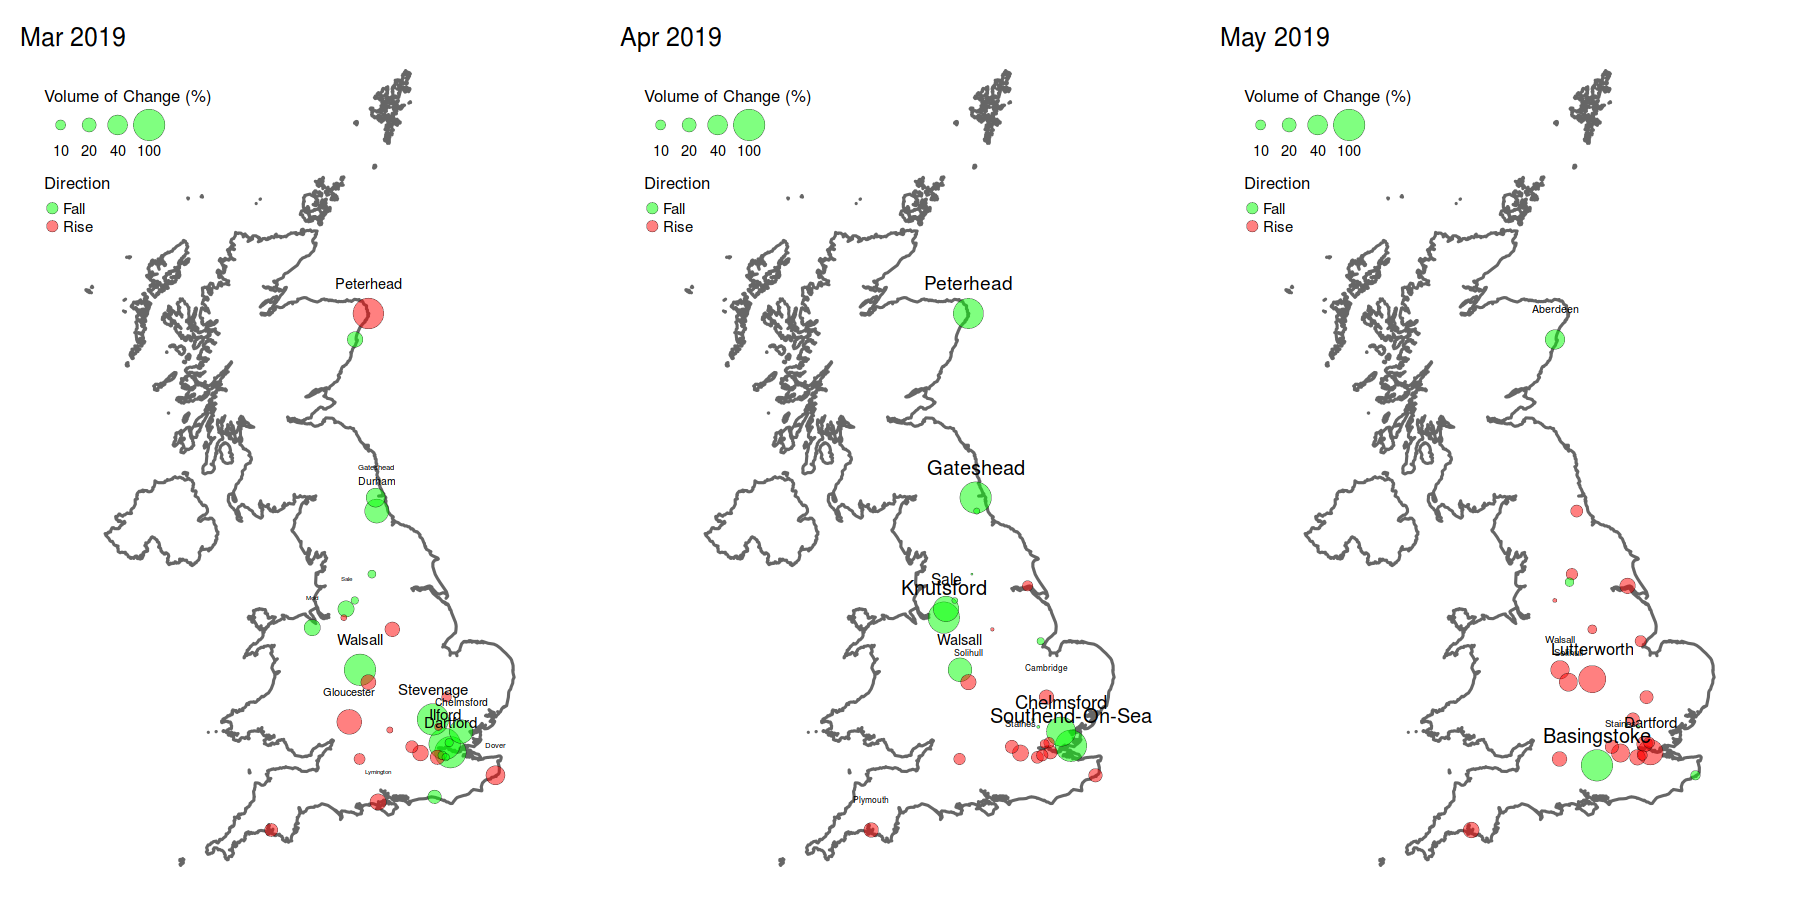
\includegraphics[trim={0 12 0 0},clip]{images/applications-city-indices.png}
  \caption{The profiles can be tracked longitudinally to reveal nature and change}
  \label{}
\end{figure*}

\begin{figure*}
  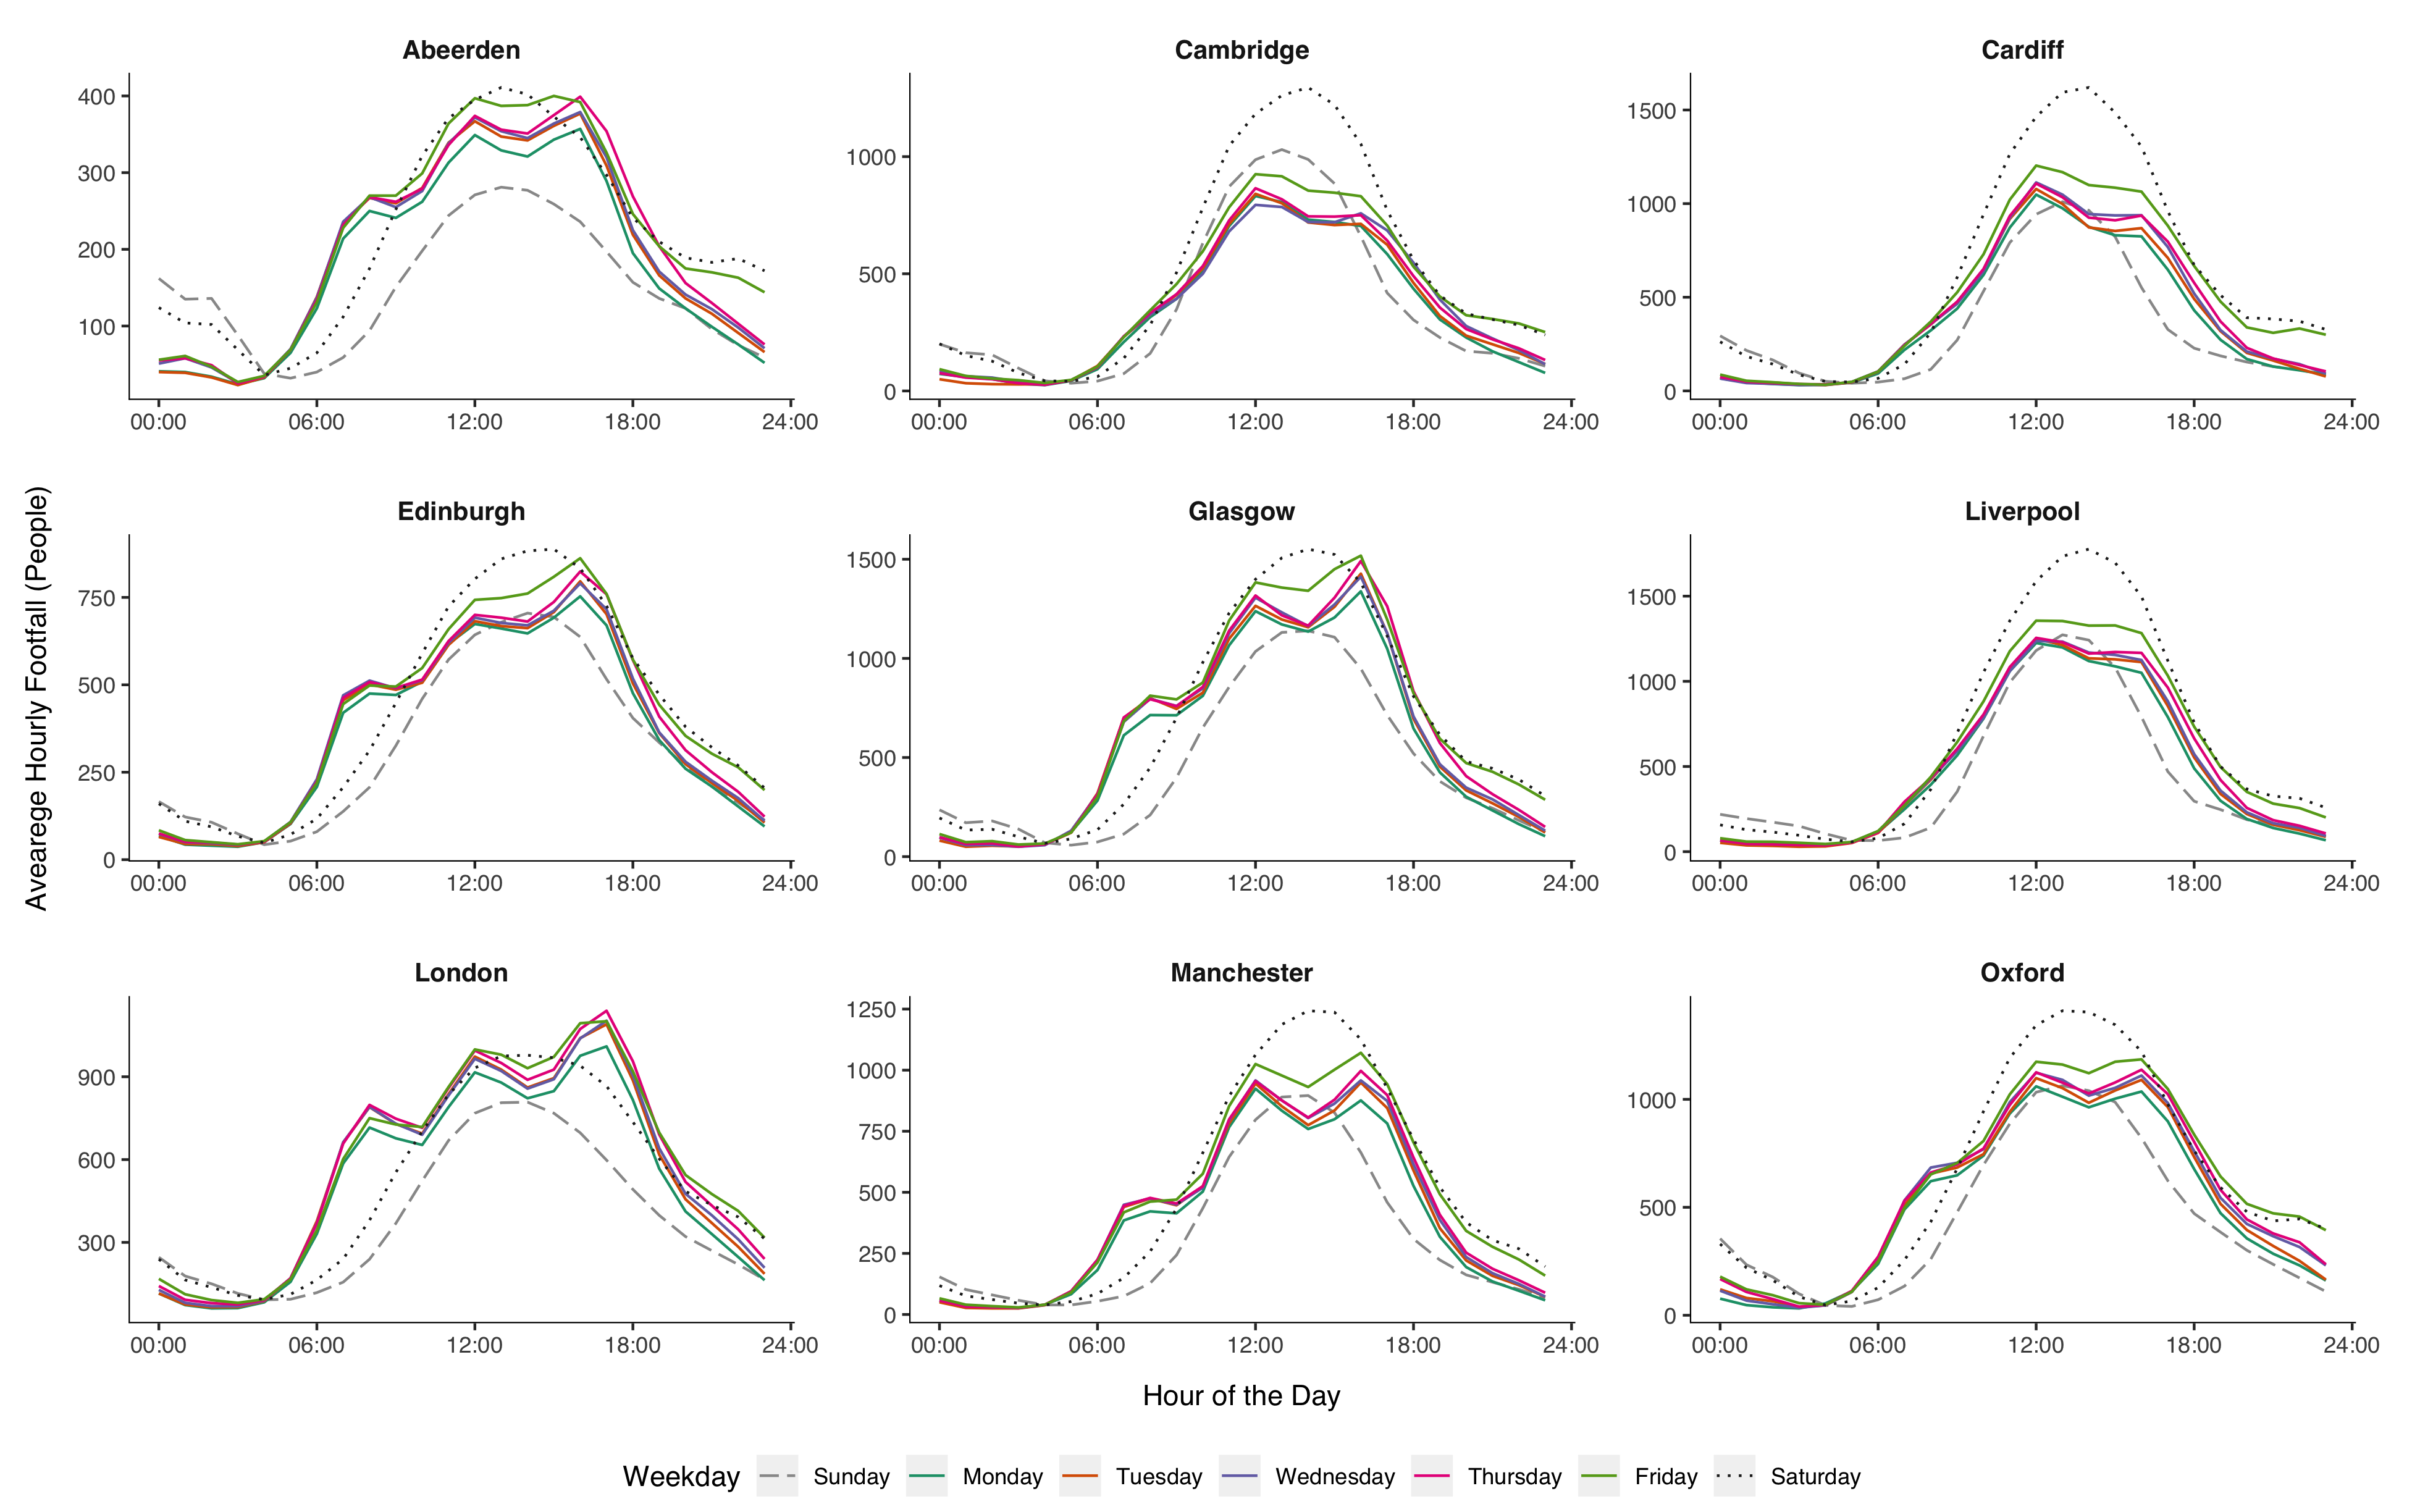
\includegraphics[trim={0 10 0 0},clip]{images/applications-city-profiles.png}
  \caption{The profiles can be tracked longitudinally to reveal nature and change}
  \label{}
\end{figure*}


\subsection{Location comparisons}
% the locations can vary widely and their profiles can show their nature. compare couple of locations to show difference in character.
\lipsum[1]

\subsection{Longitudinal analysis}
% The profiles can be tracked longitudinally to reveal nature and change of nature over time. Footfall calendar

\lipsum[1]

\cleartoleftpage
\newgeometry{
  left=20mm,
  textwidth=122mm,
  marginparsep=7mm,
  marginparwidth=43mm
}
\begin{figure*}
  \forceversofloat
  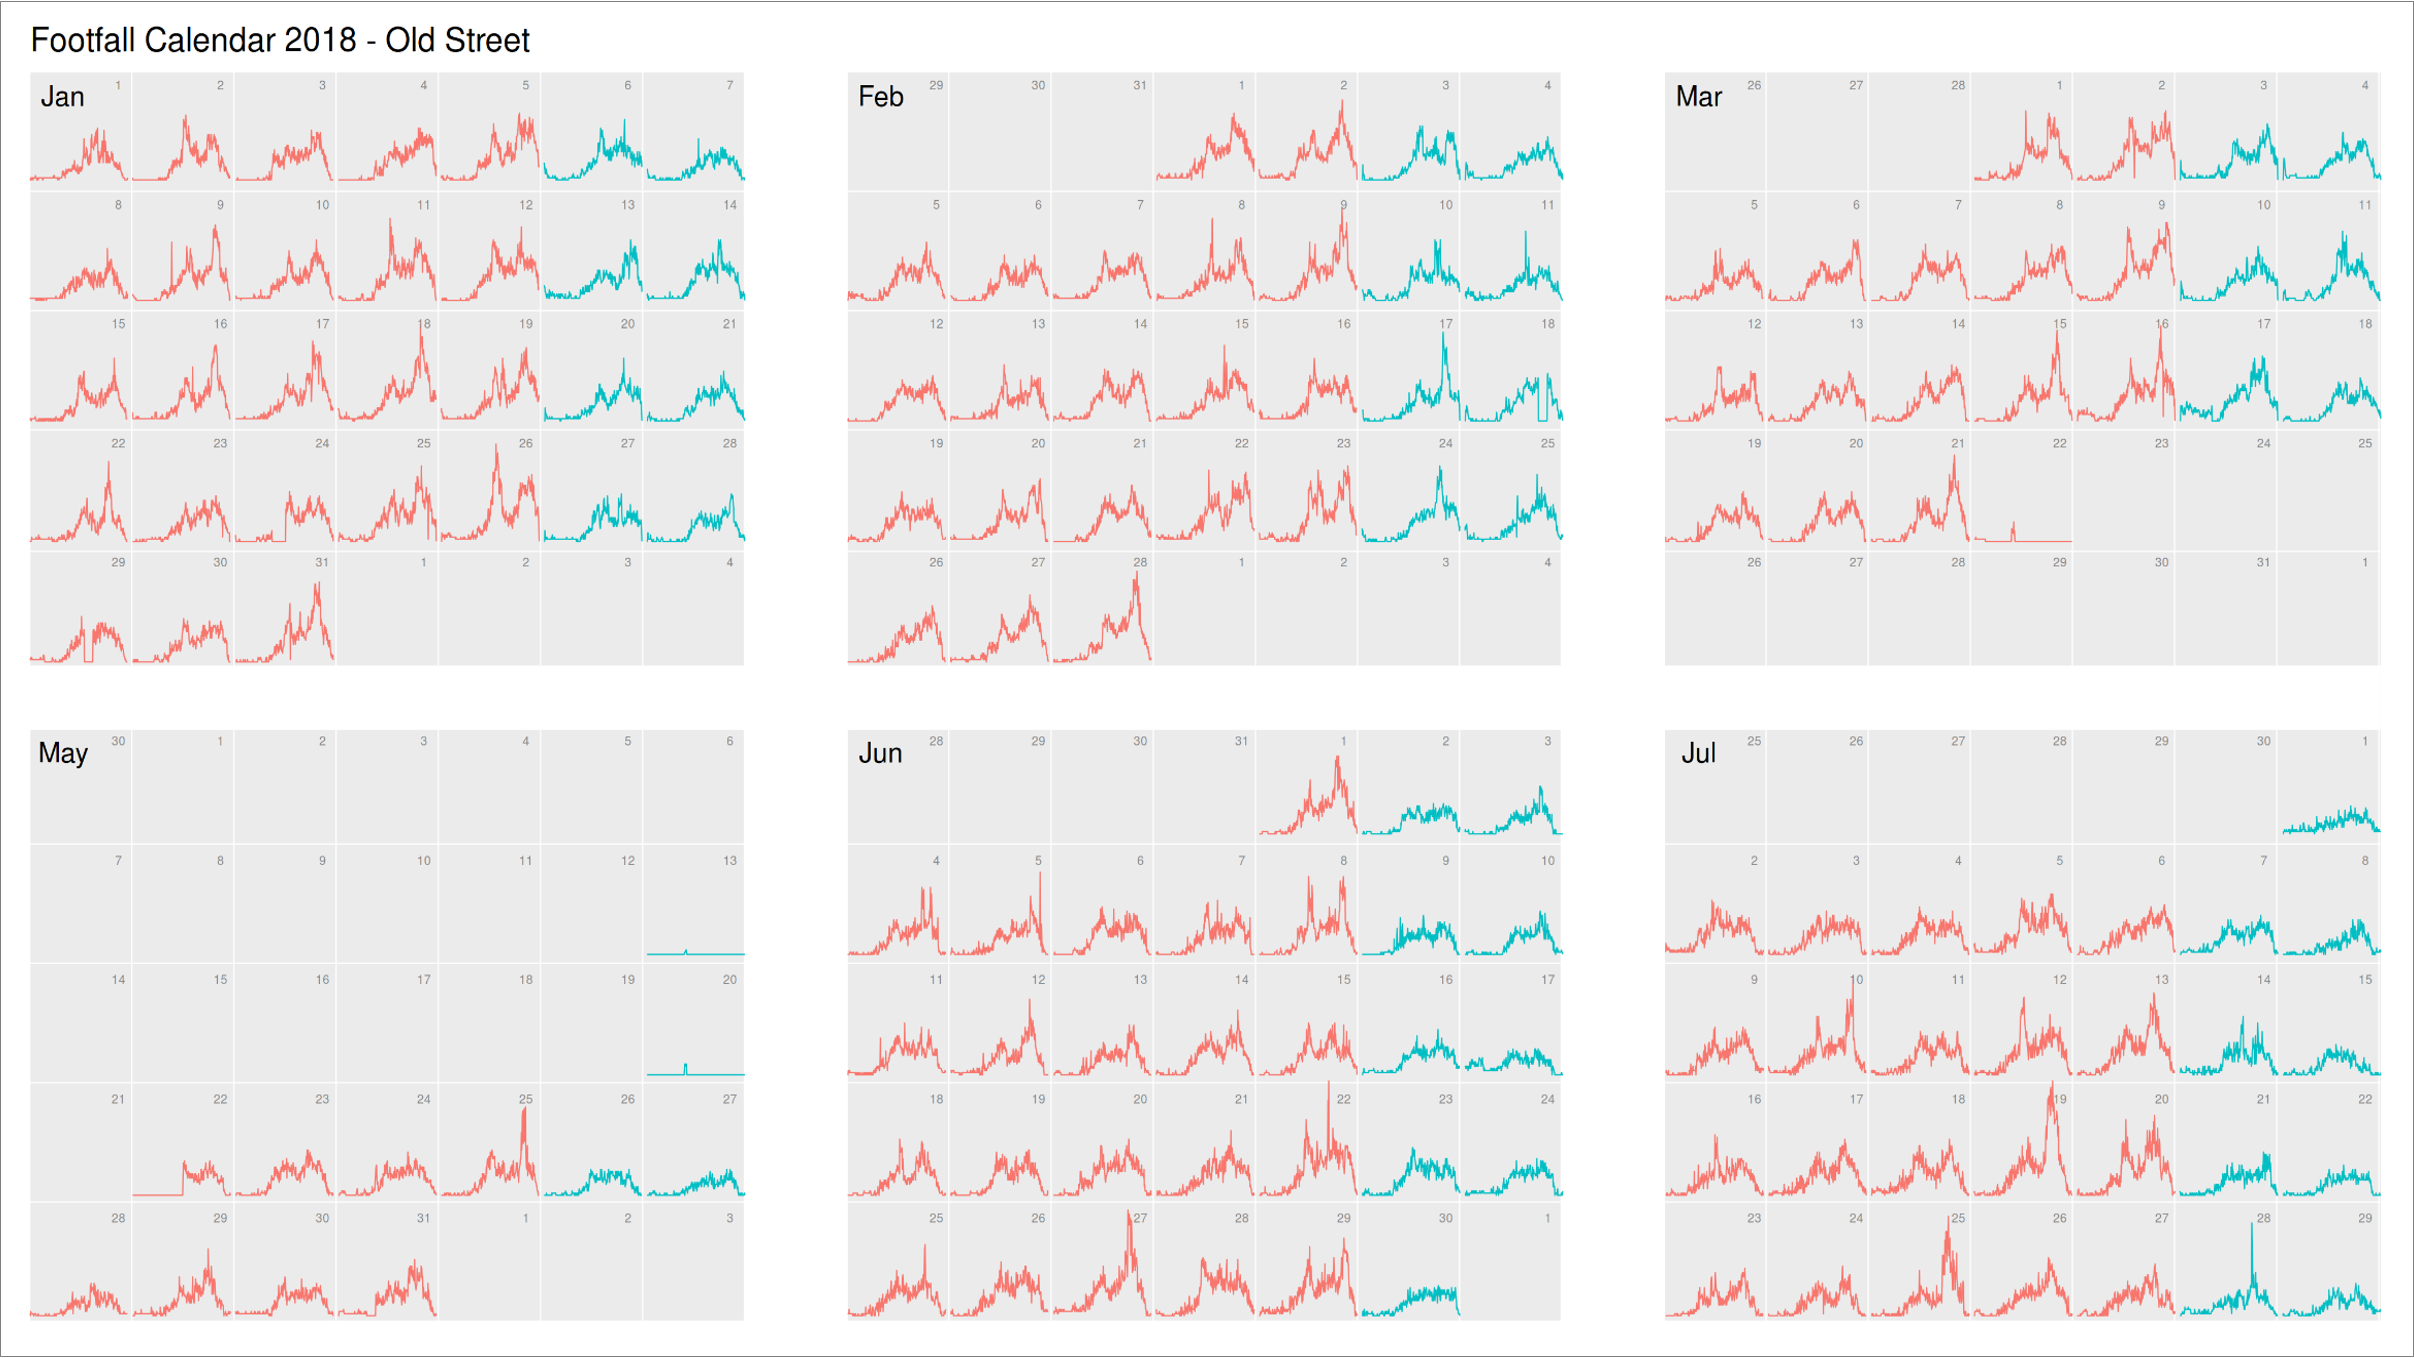
\includegraphics[width=172mm,trim={0 0 1310 -42},clip]{images/applications-footfall-calendar.png}
  \caption{Footfall calendar showing the profiles of daily volume of footfall at Old Street, London.}
  \label{}
\end{figure*}
\clearpage
\begin{figure*}
  \forcerectofloat
  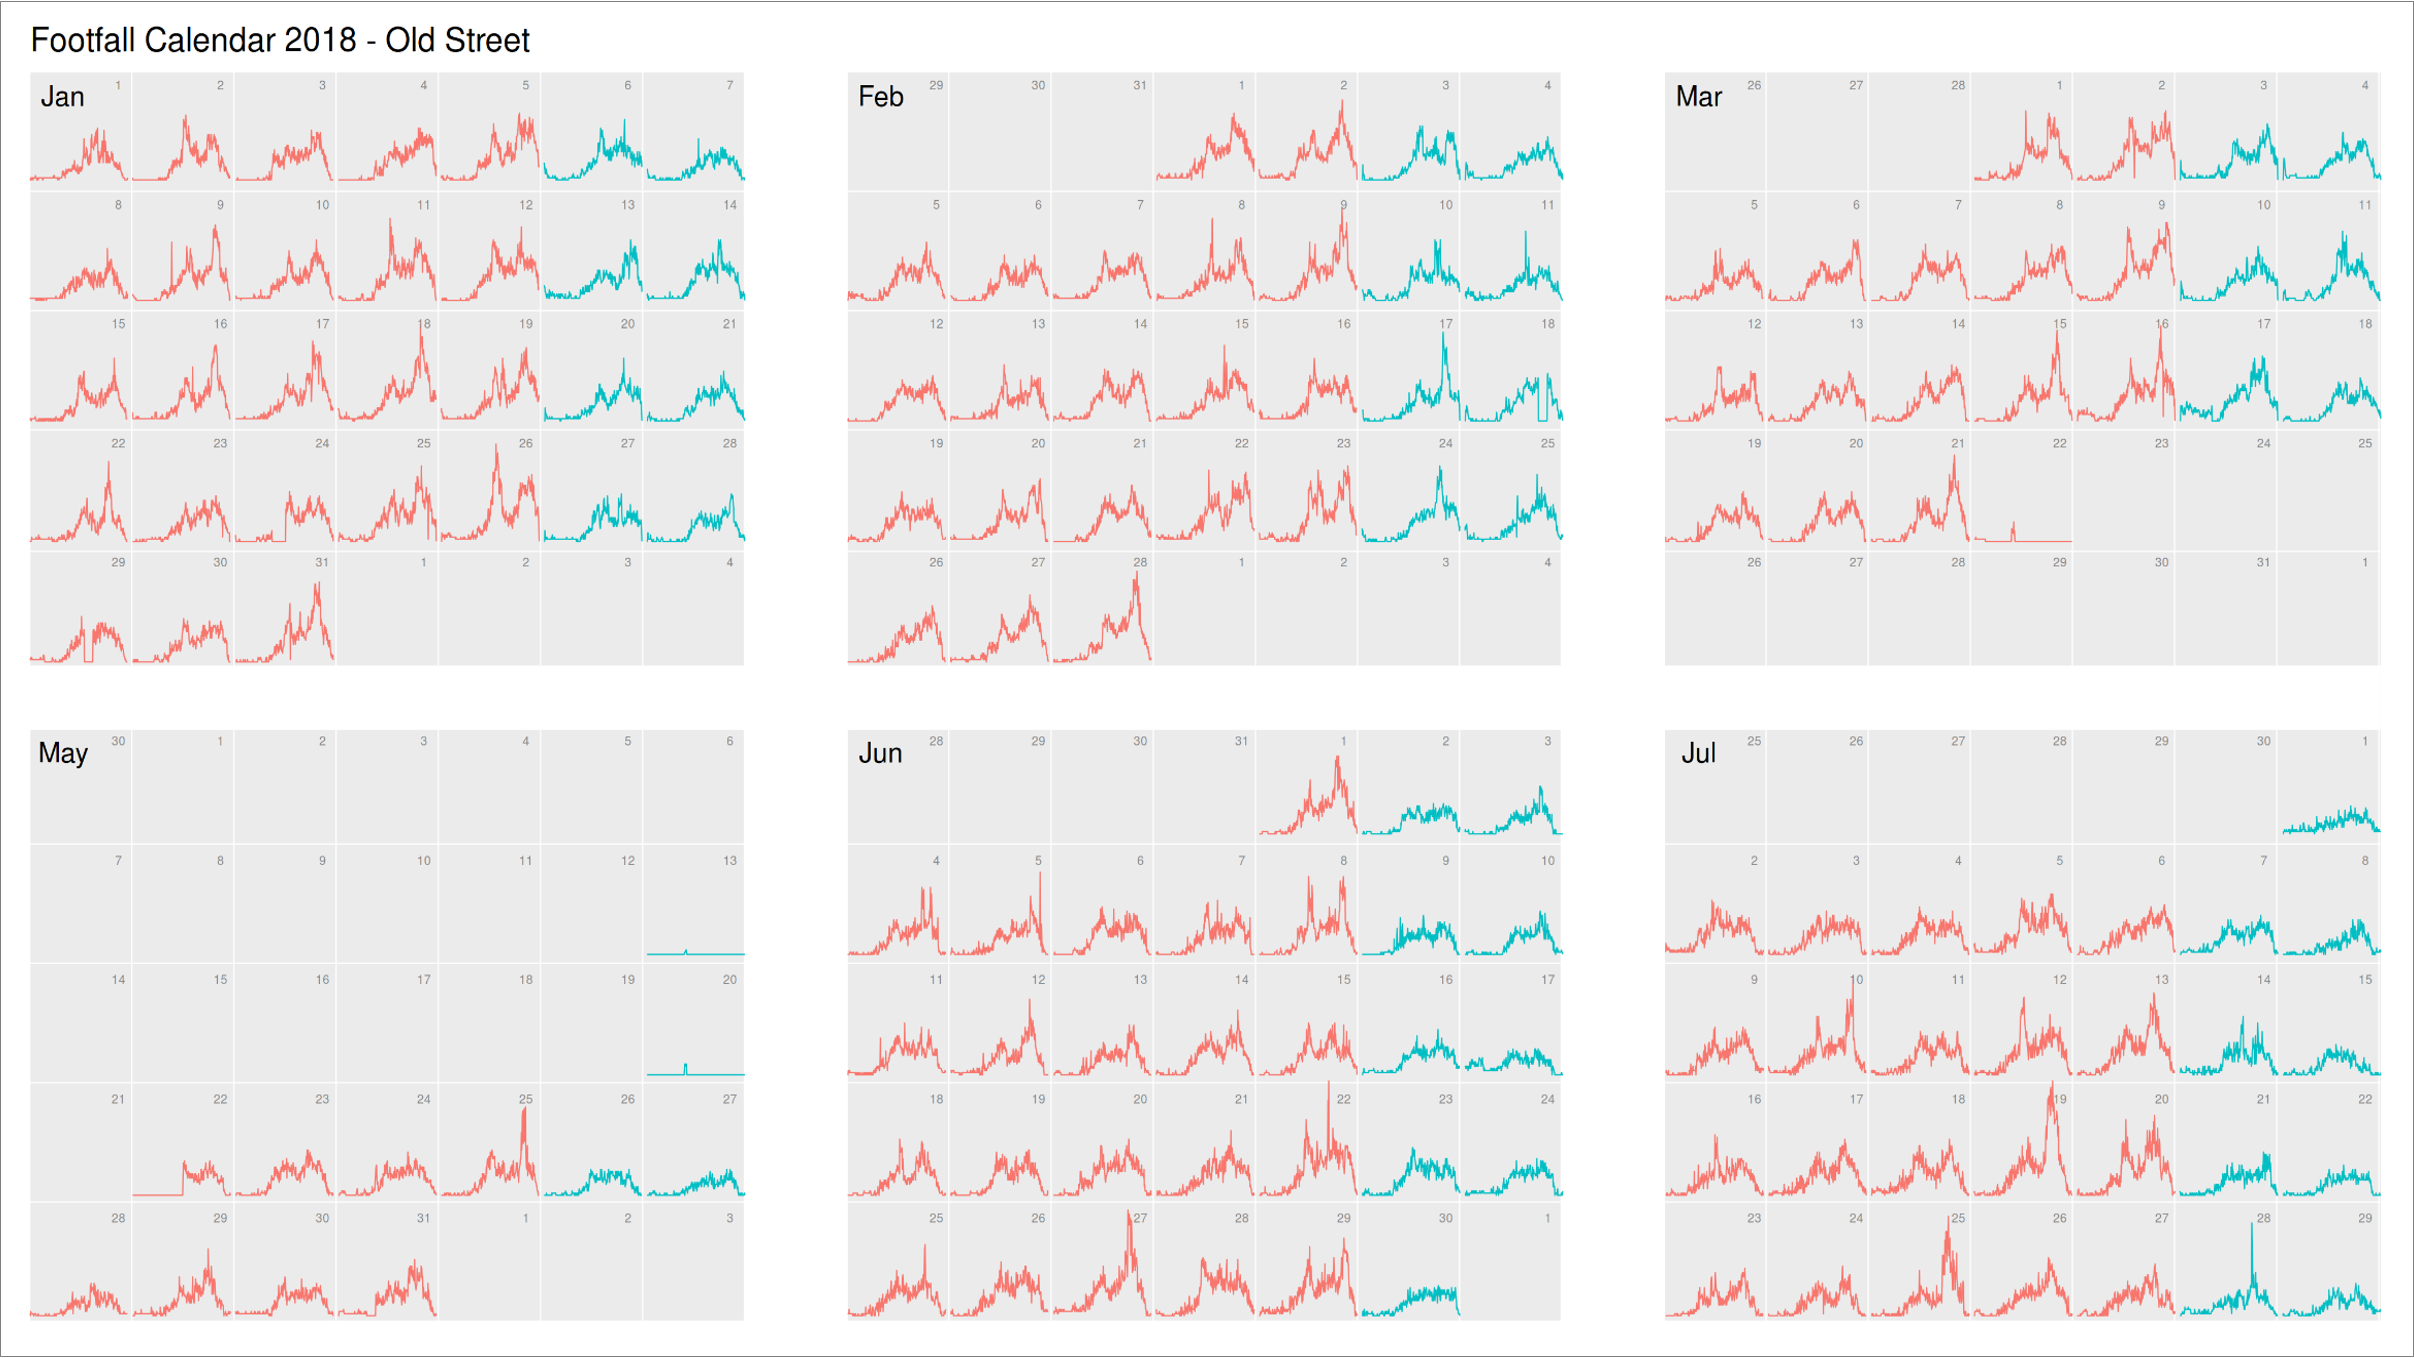
\includegraphics[width=172mm,trim={1315 0 0 0},clip]{images/applications-footfall-calendar.png}
  \caption[]{}
  \label{}
\end{figure*}
\restoregeometry
\clearpage

\lipsum[1-2]

%-------------------------------------------------------------------------------%
\section{Event Detection}
%-------------------------------------------------------------------------------%

\begin{figure*}
  \forceversofloat
  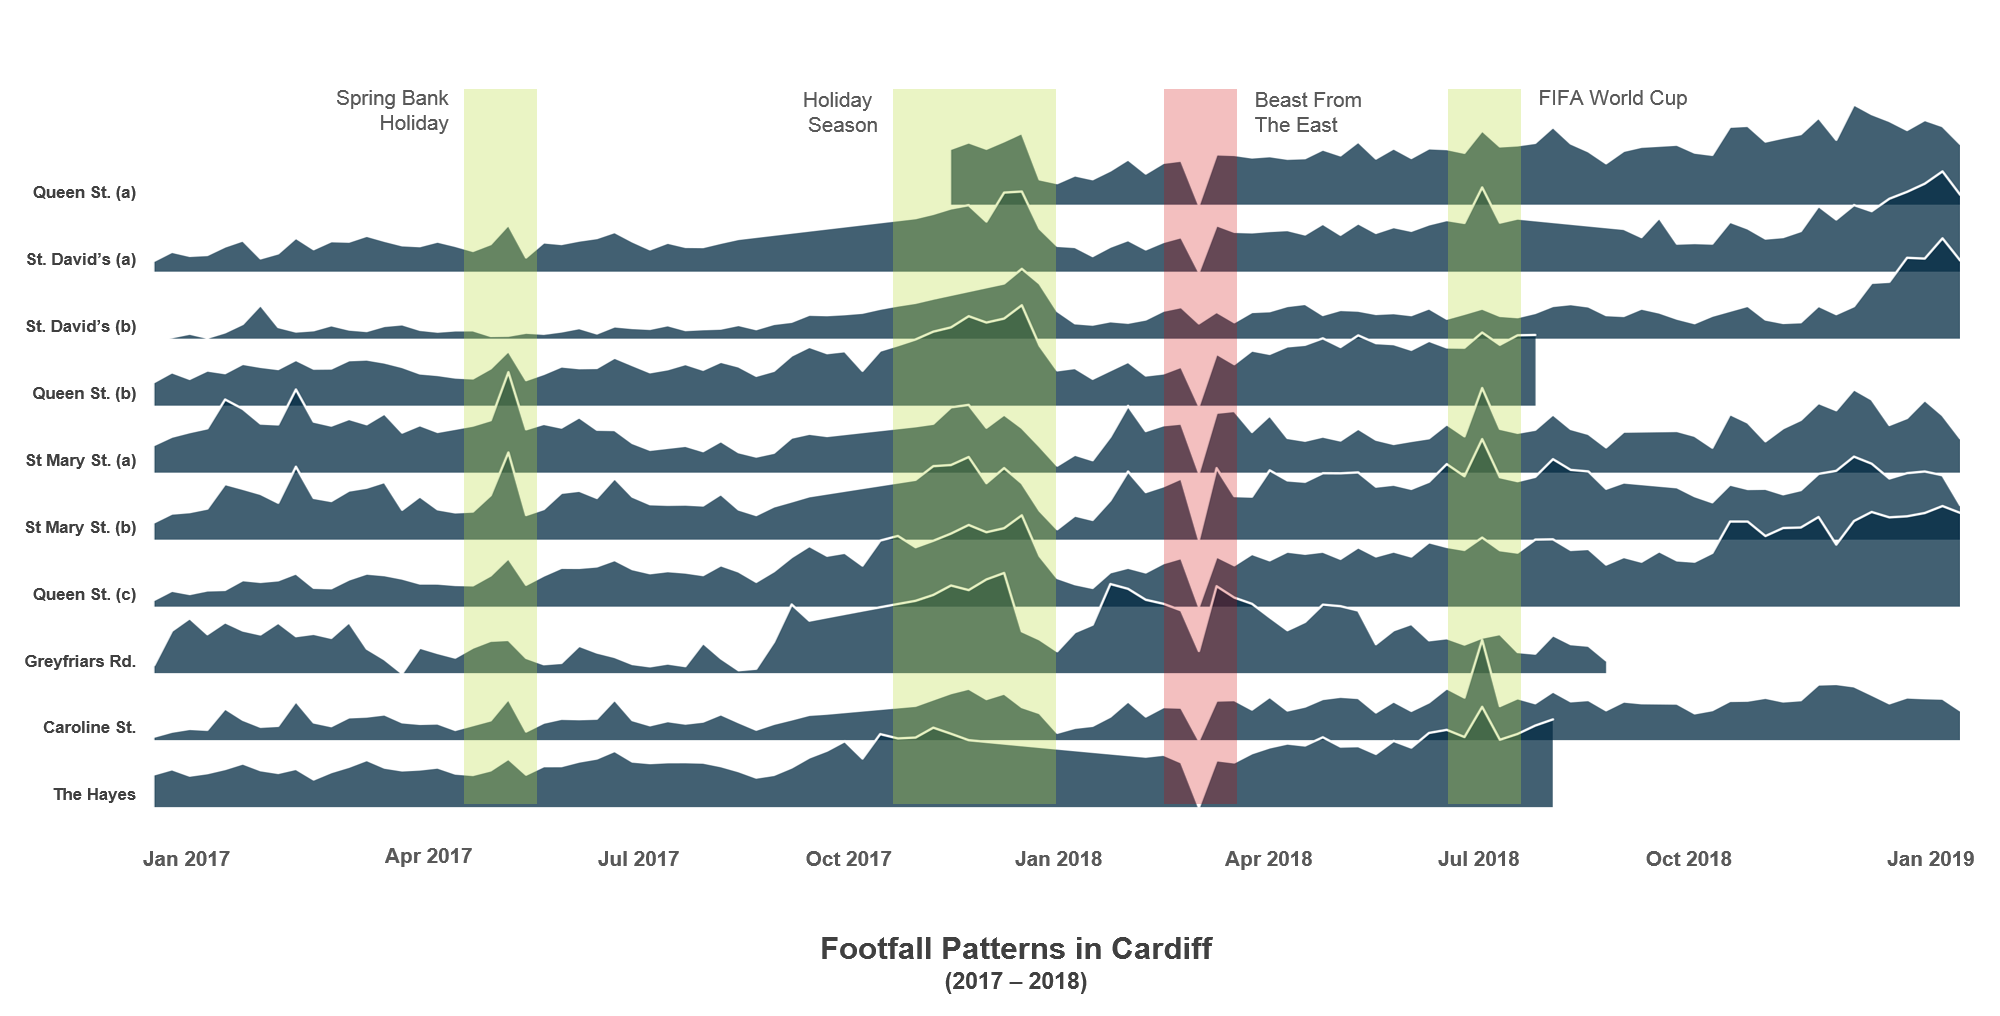
\includegraphics[trim={0 50 0 0},clip]{images/applications-cardiff-footfall.png}
  \caption{}
  \label{}
\end{figure*}

% how the data is longitudinal and can be used to detect events from the changes in footfall.
\lipsum[1]

% Discuss the events

\subsection{Football world cup}
% micro site variations could be identified as well.

% match day compared to other days.
% post match celebrations graphic.

%-------------------------------------------------------------------------------%
\section{Pedestrian Flows}
%-------------------------------------------------------------------------------%
% Tracks are a problem with this data
% But information can be extracted out of this.
% can use transfer entropy (Roberto)

\begin{figure*}
  \forceversofloat
  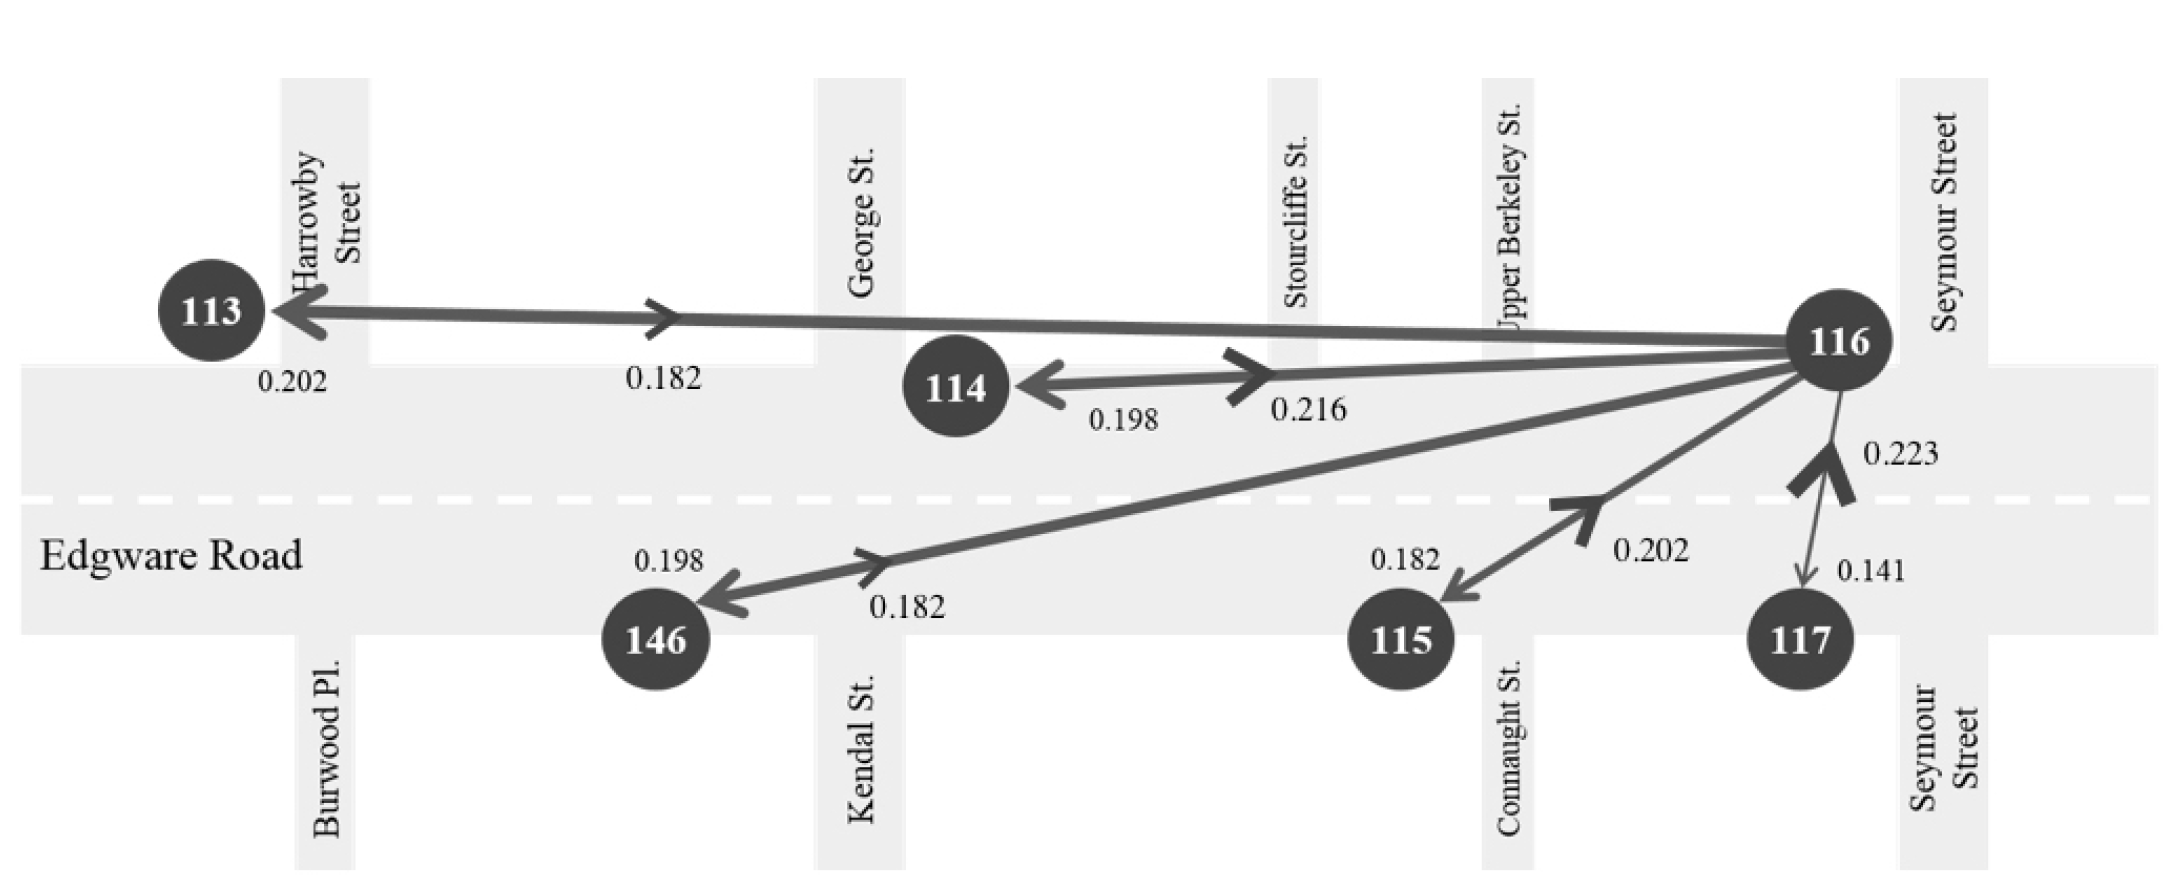
\includegraphics[trim={0 0 0 0},clip]{images/applications-transfer-entropy.png}
  \caption{}
  \label{}
\end{figure*}

% Another approach for interpolation is Geo-propagation
% It can be promising as well.

%-------------------------------------------------------------------------------%
\section{Discussion}
%-------------------------------------------------------------------------------%

% 500 words on what all the above does and how it can be taken forward.
% emphasize on other work that have been done based off this data

